\documentclass{mgragh} % opcje: robocza,man
\usepackage[cp1250]{inputenc}  % opcja latin2 dla Linuxa lub cp1250 dla Windows
\usepackage[polish]{babel}
\usepackage[OT4]{fontenc}
\usepackage{polski}
\usepackage{graphicx}

%%
%%
\makeindex 
% \includeonly{Mgr_pom,Mgr_wst,Mgr_roz1,Mgr_roz2,Mgr_lit}

%\bibliographystyle{ddabbrv}
\bibliographystyle{bibtex}
%\nocite{*}

\begin{document}
%%
%%
%% ======== METRYCZKA PRACY ========
\title{Komponentowa architektura indukcyjnej bazy danych jako platformy uczenia
maszynowego}
\author{Nikodem Jura, Krzysztof Rajda}
\promotor{dr hab. in�. Marek Kisiel-Dorohinicki}
\nralbumu{11957}
\uczelniaNazwa{Akademia G�rniczo-Hutnicza}
\uczelniaImienia{im. Stanis�awa Staszica}
\wydzial{Elektroniki, Automatyki, Informatyki i Elektrotechniki}
\kierunek{Informatyka}
\specjalnosc{In�ynieria system�w informatycznych i baz danych}
\rok{2006}

\maketitle
%%
\slowakluczowe{}

%\keywords{a,b,c,d,e,f,g,h} 
%%
%%
%% ======== NASZE MAKRA ========
%%

%----------------- nasze definicje -----------------% 
\newtheorem{stw}{\indent Stwierdzenie}[chapter]
%------------------------------%
\newcommand{\id}[1]{\index{#1}}  
\newcommand{\wi}[1]{#1\index{#1}}  
\newcommand{\wwi}[1]{\emph{#1}\index{#1}}  
\newcommand{\mwi}[1]{\textbf{#1}\index{#1}}
\newcommand{\ii}[1]{\textit{#1}}
%\newcommand{}{}

%---------------------------------------------------%



%%
%% ======== SPIS TRE�CI ========
%%
\tableofcontents
%%
%% ======== STRESZCZENIE PRACY (POLSKIE) ========
\begin{streszczenie}
%%

%--------------------------------------------------------------------%

%%
\end{streszczenie}
%%
%% ======== G��WNA CZʌ� PRACY ========
%%
%% ==== WST�P ====
%%
\begin{wstep}
%%
\section{Wprowadzenie}
%\subsection{Machine learning}
%\subsection{Indukcyjne bazy danych}
%\subsection{Zastosowania}

Integracja technologii baz danych z nowoczesnymi metodami indukcyjnego
generowania wiedzy wydaje si� dawa� istotne korzy�ci w perspektywie
budowy system�w wspomaganie decyzji. Systemy nazywane czasem
indukcyjnymi bazami danych potrafi� odpowiedzie� nie tylko na pytania,
dla kt�rych odpowied� znajduje si� w bazie danych, ale r�wnie� na
pytania, kt�re wymagaj� zsyntetyzowania i zastosowania wiarygodnej
wiedzy, wygenerowanej przez indukcyjne wnioskowanie z fakt�w z bazy
danych i wcze�niejszej wiedzy.  Indukcyjne bazy danych mog� by�
postrzegane jako naturalny krok w rozwoju system�w bazodanowych \cite{bib3}.

\begin{figure}[ht]
    \centering
        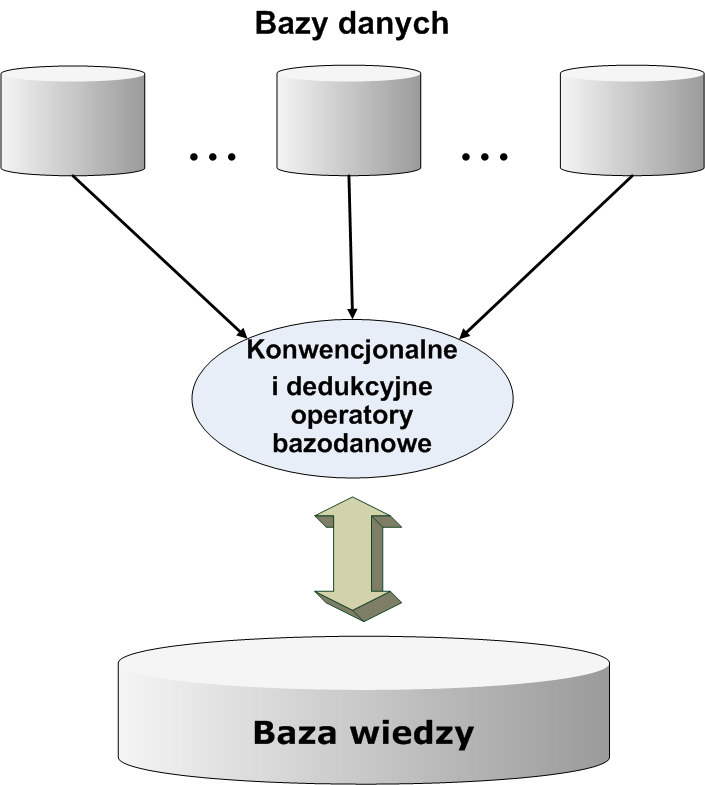
\includegraphics[width=0.70\textwidth]{img/knowledge_mining.png}
    \caption{Indukcyjne bazdy danych}
    \label{fig:architecture}
\end{figure}

\bigskip
W pracy przedstawiona zostanie architektura i wybrane aspekty
implementacji platformy \emph{Salomon}, jak r�wnie� zaprezentowane
zostan� mo�liwo�ci jego wykorzystania na przyk�adzie wybranych
algorytm�w pozyskiwania wiedzy z danych.

%\newpage
%%
\end{wstep}
%%
%% ==== ROZDZIA� 1 ====
%%
%% A tutaj tak dla przyk�adu jest \part
\part{Wprowadzenie}

%%
\chapter{Uczenie maszynowe}
%Cichosz (35-36)
\section{Algorytmy ucz�ce si�}

Pr�by opracowania algorytm�w ucz�cych si� nie wynikaj� z ch�ci wyeliminowania
projektant�w z proces�w analizy i projektowania system�w komputerowych, a wi�c
klasycznych zagadnie� in�ynierii oprogramowania. Nie mog� one bowiem by�
alternatyw� dla tradycyjnych metodologii tworzenia oprogramowania. Cele, jakie
stawiaj� sobie tw�rcy algorytm�w ucz�cych si� wynikaj� ze z�o�ono�ci niekt�rych
zagadnie� algorytmicznych -- pr�buj� oni w�a�nie za ich pomoc� opisa� te
problemy, dla kt�rych opracowanie poprawnych i pe�nych algorytm�w klasycznych
jest bardzo trudne lub wr�cz niemo�liwe.

Program ucz�cy mo�na wyobrazi� sobie jako abstrakcyjny, ,,parametryzowalny''
algorytm wykonania zadania. Proces uczenia polega na dobraniu, na podstawie
historycznych warto�ci tych ,,parametr�w'', takich warto�ci, by rozwi�zanie
spe�nia�o za�o�enia projektanta. 

,,Parametry'' te mo�na traktowa� jako pewnego rodzaju \emph{wiedz�}.
Nie s� one podawane do algorytmu w spos�b bezpo�redni (a je�li nawet s� podawane
ich pocz�tkowe warto�ci, to s� one najcz�ciej dalekie od oczekiwanych), ale
odkrywane s� przez sam algorytm podczas procesu uczenia si�.
Z tego te� powodu s� one traktowane jako wiedza niepewna i mog�ca wymaga� weryfikacji.	

Wiedza ta mo�e okre�la� zar�wno sekwencje operacji, kt�re program ma wykona�
podczas rozwi�zywania danego problemu, jak i wyb�r spo�r�d r�nych wariant�w
mo�liwych do podj�cia w danym momenecie decyzji.

Wiedza, kt�ra okre�la strategie osi�gania cel�w nazywana jest
\emph{proceduraln�}, natomiast taka, kt�ra opisuje obiekty i zwi�zki mi�dzy nimi
-- \emph{deklaratywn�}.

Algorytmy pozyskiwania i doskonalenia zdobytej wiedzy nazywane s�
\emph{algorytmami uczenia maszynowego}. 

% Cichosz 40
%\subsection{Zastosowanie algorytm�w ucz�cych}

Zastosowanie algorytm�w uczenia maszynowego jest bardzo szerokie.
Zdarza si�, �e ich wykorzystanie do rozwi�zania niekt�rych problem�w
mo�e by� tak�e podyktowane czynnikami ekonomicznymi -- czasem bardziej op�aca
si� zastosowa� algorytmy ucz�ce si�, ni� traci� czas na opracowywanie 
skomplikowanych algorytm�w klasycznych, kt�re i tak w pewnych przypadkach mog�
dzia�a� niepoprawnie.

Dla naprawd� du�ych i z�o�onych problem�w trudne jest opracowanie pe�nych i~poprawnych 
algorytm�w je rozwi�zuj�cych. Z takimi przypadkami mamy do czynienia
np. w zagadnieniach dotycz�cych realnie dzia�aj�cych system�w, w kt�rych trzeba
liczy� si� z du�� dynamik� i nieprzewidywalno�ci� �rodowiska, w kt�rym dzia�a program.
Uzyskanie poprawnie dzia�aj�cych algorytm�w pracuj�cych w takich systemach mo�e
okaza� si� bardzo kosztowne: albo ze wzgl�du na czas i �rodki potrzebne do ich
opracowania, albo ze wzgl�du na zasoby u�ywane podczas ich pracy. Zdarza si�
tak�e, ze opracowanie zadowalaj�cych algorytm�w jest wr�cz niemo�liwe.
Wynika to z tego, �e �rodowiska w kt�rych cz�sto musz� dzia�a� takie algorytmy
s� trudne do opisania -- brakuje dla nich modeli teoretycznych, lub te�
uproszczenia, kt�re musia�y zosta� w nich przyj�te, by wog�le mo�liwe by�o
opisanie danego �rodowiska nie pozwalaj� na uzyskanie wystarczaj�co dok�adnie
dzia�aj�cych algorytm�w.

W wielu zastosowaniach systemy informatyczne powinny dzia�a� mo�liwe
autonomicznie i wymaga� znikomej ingerencji ze strony cz�owieka. Przyk�adami
takich system�w mog� by� systemy kontroli poszczeg�lnych instalacji w
nowoczesnych biurowcach, systemy sterowania robotami przemys�owymi czy pojazdami
bezza�ogowymi. Wymagany stopie� autonomii tych system�w jest niemo�liwy do
uzyskania bez wyposa�enia ich w mo�liwo�� adaptacji, czyli przystosowania si� do
zmieniaj�cych si� warunk�w. Systemy posiadaj�ce zdolno�� adaptacji mog� by�
u�ywane w nieprzewidywalnym �rodowisku lub wielu podobnych �rodowiskach.

Jednym z najwa�niejszych zastosowaniem algorytm�w ucz�cych jest nowoczesna
analiza danych, tzw. \emph{data mining}.
Wsp�czesne zbiory danych, kt�re musz� by� poddawane analizie pochodz� np.
z d�ugotrwa�ych pomiar�w i eksperyment�w naukowych. Zawieraj� ogromne ilo�ci
danych, co powoduje, ze nie mog� one by� analizowane w inny spos�b, ni�
automatycznie. Do ich filtrowania i wyszukiwania zale�no�ci mi�dzy nimi
wykorzystuje si� specjalnie opracowane algorytmy, kt�re potrafi� nie tylko
przetwarza� dane aktualne, ale tak�e wnioskowa� na podstawie danych historycznych,
przechowywanych w ogromnych bazach danych, zwanych \emph{hurtowniami danych}.

%Troche przykladow
\subsection{Metody reprezentacji wiedzy}

% Cichosz 41-42
Wiedza z punktu widzenia algorytm�w ucz�cych mo�e by� przechowywana na r�ne
sposoby -- opracowano w tym celu wiele efektywnych struktur danych,
pozwalaj�cych na jej �atwe zapisanie i przetwarzanie.
Z regu�y jednak dziedzina, w jakiej ma byc wykorzystany algorytm ucz�cy,
determinuje, lub w najlepszym przypadku zaw�a, ilo�� mo�liwych reprezentacji
wiedzy, z kt�rych ka�da ma swoje dobre strony jak i ograniczenia.
Do podstawowych metod reprezentacji wiedzy nale�� drzewa decyzyjne, formu�y
logiki predykat�w, wykorzystuje si� tak�e rozk�ady prawdopodobie�stwa oraz
automaty sko�czone.

Jednym z podzia��w metod reprezentacji wiedzy jest rozr�nienie mi�dzy metodami
\emph{symbolicznymi} i \emph{subsymbolicznymi}.
Metody symboliczne do reprezentacji wiedzy stosuj� struktury przechowywuj�ce
informacje o chartakterze symbolicznym, czyli pewne napisy, kt�re mog� by� w
pewien spos�b interpretowane. Napisy te najcz�ciej maj� form� czyteln� dla
cz�owieka i mog� by� przez niego przegl�dane i poddawane analizie i
interpretacji. 
Metody drugiej z kategorii przechowuj� informacje w formie trudnej do
interpretacji przez cz�owieka. Poszczeg�lne dane analizowane
pojedynczo nie nios� �adnej sensownej informacji, gdy� cz�sto s� to ci�gi liczb
lub dane binarne. Dopiero odpowiednio po��czone ze sob� dane poddane
przetwarzaniu reprezentuj� pewn� wiedz�.

Nie zawsze metoda u�yta do reprezentacji wiedzy dla okre�lonych zastosowa� jest
jedynym mo�liwym sposobem jej przedstawienia, jednak rzadko zdarza si�, by wyb�r
metody by� szeroki. Wynika to z tego, �e spos�b, w jaki wiedza mo�e by� u�yta
zale�y g��wnie od wyboru metody oraz celu, czyli zadania, kt�re ma by� wykonane
przez algorytm ucz�cy.

Do najpowszechniejszych zada�, kt�re stawia si� przed algorytmami ucz�cymi
nale�� klasyfikacja i aproksymacja. Klasyfikacja ma na celu ustalenie
przynale�no�ci danych obiekt�w do okre�lonych kategorii, natomiast aproksymacja
polega na odzworowaniu obiekt�w na zbi�r liczb rzeczywistych.

Algorytmy ucz�ce mog� tak�e by� wykorzystane do innych zastosowa�, jak np.
sekwencyjne podejmowanie decyzji, czy te� modelowanie z�o�onych �rodowisk, dla
kt�rych opracowanie klasycznych modeli jest trudne, lub nawet niemo�liwe.
Znajduj� one tak�e zastosowanie jako narz�dzia wspomagaj�ce cz�owieka w
przetwarzaniu du�ej ilo�ci informacji -- mog� one przedstawia� wiedz� uzyskan� z
analizy du�ej ilo�ci danych w bardziej czytelnej dla cz�owieka formie.

% Cichosz 43-44
\subsection{Podzia� algorytm�w ucz�cych}

Jednym z najbardziej podstawowych kryteri�w podzia�u algorytm�w ucz�cych si� jest
ich podzia� na  \emph{uczenie si� z nadzorem} i \emph{bez nadzoru}.

W przypadku uczenia z nadzorem (czasami nazywanego tak�e \emph{uczeniem z
nauczycielem}) wiedza uzyskiwana w czasie dzia�ania algorytmu ucz�cego jest
weryfikowana -- algorytm dla okre�lonych danych wej�ciowych otrzymuje tak�e
oczekiwane informacje wyj�ciowe, zwane \emph{informacj� trenuj�c�}.
Zadaniem procesu uczenia si� jest takie dobranie parametr�w algorytmu, aby dla
okre�lonych danych wej�ciowych otrzyma� dane wyj�ciowe mo�liwie zbli�one do
wzorcowych.

W procesie uczenia bez nadzoru nie jest dost�pna informacja trenuj�ca. Podawane
s� jedynie dane wej�ciowe i jedynie na ich podstawie algorytm ma si�
,,nauczy�'' prawid�owo je interpretowa�. Z takimi przypadkami mamy do czynienia
g��wnie w algorytmach grupuj�cych obiekty, gdzie nie s� znane kryteria, wed�ug
kt�rych obiekty maj� zosta� pogrupowane. Czasem m�wi si�, �e takie algorytmy
maj� wbudowanego nauczyciela, jako �e weryfikacja uzyskiwanej wiedzy jest
integraln� cz�ci� algorytmu.

Uczenie z nauczycielem i bez nadzoru to najbardziej popularne grupy algorytm�w,
jednak wyr�nia si� tak�e inne. Podobn� do uczenia z nadzorem grup� algorytm�w
s� metody \emph{uczenia na podstawie zapyta�}. W takim przypadku informacja
trenuj�ca co prawda pochodzi od nauczyciela, lecz stanowi jedynie odpowied� na
zadane przez ucznia pytanie. W odr�nieniu od uczenia pod nadzorem, nauczyciel
nie podaje przyk�ad�w danych wej�ciowych i oczekiwanych odpowiedzi, a jedynie
odpowiada na jawne pytanie ucznia.

Mo�na tak�e wyr�ni� metod� \emph{uczenia przez eksperymentowanie}. Mamy z ni�
do czynienia, gdy algorytm gromadzi wiedz� poprzez wykonywanie eksperyment�w ze
�rodowiskiem, w kt�rym dzia�a. Polega to na wykonywaniu pewnych dzia�a�, a
nast�pnie obserwowaniu ich konsekwencji i wp�ywu, jakie maj� one na �rodowisko.

Zbli�on� to uczenia przez eksperymentowanie metod� jest \emph{uczenie ze
wzmocnieniem}. Podobnie jak poprzednia metoda opiera si� ono na
eksperymentowaniu, jednak wykorzystuje dodatkowo pewn� informacj� trenuj�c�,
pozwalaj�c� na ocen� uzyskanej wiedzy. W tym przypadku informacja ta nie 
ma charakteru instrukta�owego, ale pozwala na otrzymanej warto�ciowanie wiedzy
poprzez przypisanie jej liczbowych wsp�czynnik�w zwanych \emph{wzmocnieniami}.
Pozwala to na ocen� dotychczasowego przebiegu procesu uczenia si� i dobieranie
jego parametr�w tak, by uzyskiwana by�a wiedza zbli�ona do tej z najwy�szymi wsp�czynnikami. 

\subsection{Metody uczenia si�}

% Cichosz 44
Informacja trenuj�ca stanowi dla algorytmu ucz�cego si� podstaw�, kt�r�
wykrzystuje do nabywania nowej wiedzy lub do udoskonalenia ju� posiadanej.
Reprezentacja tej wiedzy oraz spos�b jej wykorzystania najcze�ciej
podporz�dkowany jest zadaniu, do realizacji kt�rego ma zosta� u�yta.
Mechanizm odkrywania nowej lub ulepszania ju� posiadanej wiedzy z regu�y mocno
zale�y od sposobu jej reprezentacji oraz postaci informacji trenuj�cej.

Z regu�y do realizacji konkretnego mechanizmu zdobywania wiedzy mog� by� u�yte
r�norodne algorytmy.
Najbardziej popularn� metod� uczenia si� jest \emph{indukcja}. Polega ona na
wnioskowaniu na podstawie posiadanej, konkretnej, informacji trenuj�cej. Ma ona
na celu celu uzyskania wiedzy og�lnej za pomoc� uog�lnienia informacji
trenuj�cej na pozosta�e przypadki.

Opr�cz metod indukcyjnych, wyr�nia si� tak�e mechanizmy \emph{uczenia
nieindukcyjnego}. Metody te maja na celu nie tyle wnioskowanie, ile raczej 
wyja�nianie -- informacja trenuj�ca nie jest uog�lniania, lecz wykorzystywana
jest do konkretyzacji ju� zdobytej przez algorytm ucz�cy si� wiedzy.
% Add reference here - uczenie ze wzmocnieniem
Do metod tych zalicza si� tak�e stosowane przy uczeniu ze wzmocnieniem
warto�ciowanie zdobytej wiedzy pozwalaj�ce na lepsze wyselekcjonowanie
po�ytecznej wiedzy.

%Cichosz 45 - glowne dzialy uczenia maszynowego
\subsection{G��wne nurty uczenia maszynowego}

Badania nad r�nymi systemami ucz�cymi doprowadzi�y to powstania nowej dziedziny
naukowej -- \emph{uczenia maszynowego}. Dziedzina ta mo�e by� traktowana jako
ga��� sztucznej inteligencji, czy szerzej -- informatyki.
W zg��bianie zagadnie� uczenia maszynowego zaanga�owani s� nie tylko
informatycy, co wydaje si� naturalne, ale tak�e przedstawiciele innych dziedzin
takich jak matematyka, a nawet psychologia, czy biologia.

%za Cichoszem
Wydziela si� 3 g��wne nurty, w kt�rym zmierzaj� prace badawcze w dziedzinie
uczenia maszynowego -- nurt \emph{teoretyczny}, \emph{biologiczny} i \emph{systemowy}.

Badacze zajmuj�cy si� nurtem teoretycznym stawiaj� sobie za cel przede
wszystkim rozwijanie podstaw teoretycznych, na kt�rych ma opiera� si� ca�a
dziedzina. Staraj� si� oni nazwa� i usystematyzowa� poj�cia zwi�zane z t�
dziedzin� i d��� do utworzenia s�ownika poj�� teoretycznych, kt�ry by�by
powszechnie wykorzystywany przez wszystkich zajmuj�cych si� uczeniem maszynowym.
Opr�cz opracowywania podstaw teoretycznych zajmuj� si� tak�e przyk�adowo 
klasyfikacj� problem�w, kt�rymi zajmuje si� uczenie maszynowe, ze wzgl�du na ich
trudno��, czy te� okre�laniem wp�ywu ilo�ci informacji trenuj�cej na szybko��
procesu uczenia si�.

Nurt biologiczny zajmuje si� opracowywaniem modeli obliczeniowych proces�w uczenia si�
wyst�puj�cych w przyrodzie, czyli na przyk�ad u ludzi i zwierz�t. Modele te
tworzone s� na r�nym poziomie szczeg�owo�ci, pocz�wszy od pojedy�czych kom�rek
a na z�o�onych uk�adach nerwowych sko�czywszy.

Z informatycznego punktu widzenia, najbardziej interesuj�cym nurtem jest nurt
systemowy. W odr�nieniu od nurtu biologicznego, kt�rym cz�sto zajmuj� si� te�
biolodzy czy psycholodzy, nurtem systemowym zajmuj� si� g��wnie informatycy i
jest to nurt dominuj�cy w dziedzinie uczenia maszynowego. 
Jego g��wnym celem jest opracowywanie algorytm�w uczenia maszynowego oraz
badaniem ich wykorzystania w systemach ucz�cych.

% Cichosz 56-57
\subsection{Zastosowanie system�w ucz�cych si�}

Nie ulega w�tpliwo�ci, �e nawet tak stosunkowo m�oda dziedzina informatyki, jak�
jest uczenie maszynowe, znajduje ju� praktyczne zastosowania.

\subsubsection{Wydobywania wiedzy z baz danych}

Jednym z g��wnych zastosowa� system�w ucz�cych jest ich wykorzystanie do
wydobywania wiedzy z baz danych. W du�ych systemach informatycznych
przechowywane s� niewyobra�alne ilo�ci danych i potrzebne s� narz�dzia
wspomagaj�ce ich efektywne przetwarzanie. W odr�nieniu od zwyk�ych system�w
pozwalaj�cych na przeszukiwanie danych, systemy ucz�ce pozwalaj� dodatkowo na
analiz� tych danych poprzez znajdowanie zwi�zk�w i zale�no�ci miedzy nimi, co
prowadzi do pozyskania dodatkowej wiedzy, nie zapisanej bezpo�rednio w danych.

Takie zastosowanie system�w ucz�cych mo�e przynosi� bardzo konkretne korzy�ci
instytucjom z nich korzystaj�cych, przyk�adowo bank mo�e wykorzysta� dane
historyczne do analizy ryzyka kredytowego dla klienta, minimalizuj�c w ten
spos�b prawdopodobie�stwo udzielenia niekorzystnego kredytu. 
Zak�ady produkcyjne mog� za pomoc� system�w ucz�cych optymalizowa� proces
produkcji towar�w, minimalizuj�c koszty i maksymalizuj�c wydajno��.
Systemy takie znajduj� nie tylko zastosowania w biznesie, ale tak�e w nauce.
Metody uczenia maszynowego wykorzystywane s� na przyk�ad przez chemik�w do
wyszukiwania ukrytych regularno�ci w zbiorach danych analitycznych oraz 
do prognozowania wybranych w�a�ciwo�ci zwi�zk�w organicznych.

Systemy ucz�ce nie tylko mog� dostarcza� wymiernych korzy�ci finansowych, ale
tak�e mog� pomaga� ratowa� ludzkie �ycie. Analiza bazy danych zawieraj�cej
historie chor�b wspomaga lekarza w udzieleniu trafnej diagnozy choremu
pacjentowi.

Najwieksz� baz� danych jest dzi� Internet. Trudno wyobrazi� sobie 
�ycie bez wyszukiwarek, kt�re musz� analizowa� ogromne ilo�ci danych oraz
potrafi� wyszuka� zale�no�ci mi�dzy nimi. To tak�e jest obszar, w kt�rym
znajduj� zastosowanie systemy ucz�ce.

\subsubsection{Inteligentne maszyny}

- inteligentne sterowanie
- brzmi jak science-fiction
- intelig. sterowane budyntki
- systemy w samochodach - wspomagajace kierowce (pomagaja w prowadzeniu auta,
 staraja sie na podstawie warunkow ocenic, czy kierowca dobrze robi, nawet
 awartyjnie zachamowac, lub przygotowac sie do nieuniknionego zderzenia --
 napinacze pasow, usztywnienie oparcja itp.)
 Dostosowanie sie do stylu jazdy kierowcy (skrzynie przewidujace nastepny ruch kierowcy
 - w Ferrari Enzo :-)
 - robociki - ladowniki kosmiczne, robociki grajace w pilke, gry - inteligentni
 przeciwnicy, nie tylko w prostych grach (szachy) ale bardziej zlozonych grach
 strategicznych. (zlozonosc i zmiennosc srodowisk, w ktorych dzialaja) 
 	
\subsubsection{In�ynieria oprogramowania TODO:}

- inteligentne interfejsy uzytkownika (adaptujace sie do uzytka, domyslnie
wypelniajace sie pola, wykonywanie tych samych sekwencji polecen)

- projektowanie systemow - np. do estymowania kosztow nowego projektu na
podstwie analizy danych historycznych dotyczacych podobnych projetkow
(czasochlonnosc, ile ludzi w poszczegolnych okresach) - pozwala na
efektywniejsze zaplanowanie a wiec na mniejsze ryzyko niedotrzymania terminow
albo klapy biznesowej


\section{Drzewa decyzyjne}
% http://www.dbmsmag.com/9807m05.html
% When a businessperson needs to make a decision based on several factors, a
% decision tree can help identify which factors to consider and how each factor
% has historically been associated with different outcomes of the decision. For
% example, in our credit risk case study (See the sidebar Predicting Credit Risk),
% we have data for each applicant�s debt, income, and marital status. A decision
% tree creates a model as either a graphical tree or a set of text rules that can
% predict (classify) each applicant as a good or bad credit risk.

Kiedy biznesmen potrzebuje podj�� decyzje bazuj�c na kilku wsp�czynnikach,
drzewa decyzyjne mog� pomoc w wybraniu odpowiednich wsp�czynnik�w oraz 
opowiedzie� jak dany wsp�czynnik w przesz�o�ci wp�ywa� na decyzje.
Przyk�adowo, podczas obliczania ryzyka kredytowego, posiadamy dla ka�dego
potencjalnego kredytobiorcy dane o jego kredytach, przychodach oraz jego
statusie materialnym. Drzewa decyzyjne tworz� zar�wno drzewo w postaci
graficznej, jak zbi�r regu� tekstowych, dzi�ki kt�rym mo�emy okre�li�,
czy dana aplikacja jest obarczona du�ym lub ma�ym ryzykiem kredytowym.

% A decision tree is a model that is both predictive and descriptive. It is called
% a decision tree because the resulting model is presented in the form of a tree
% structure. (See Figure 1.) The visual presentation makes the decision tree model
% very easy to understand and assimilate. As a result, the decision tree has
% become a very popular data mining technique. Decision trees are most commonly
% used for classification (predicting what group a case belongs to), but can also
% be used for regression (predicting a specific value).

Drzewo decyzyjne jest modelem, kt�ry jest zar�wno predyktywnym!!!predictive and
descriptive!!!.
Nazywany jest drzewem decyzyjnym, poniewa� prezentowany jest w formie
drzewiastej struktury~\ref{fig:sample_tree}. Graficzna reprezentacja powoduje,
�e zrozumienie go czy por�wnanie go nie jest trudnym zadaniem. Drzewa decyzyjne
sta�y si� bardzo popularne w technikach ,,data maning''. Drzewa decyzyjne s�
najpowszechniej u�ywane do klasyfikacji (predykuj� do kt�rej grupy nale�y dany
przypadek), lecz mog� by� r�wnie� u�ywane przy regresji (predykuj� warto��).

% The decision tree method encompasses a number of specific algorithms, including
% Classification and Regression Trees (CART), Chi-squared Automatic Interaction
% Detection (CHAID), C4.5 and C5.0 (from work by J. Ross Quinlan of Rulequest
% Research Pty Ltd, in St. Ives, Australia, www.rulequest.com).

Metody drzew decyzyjnych obejmuj� wiele algorytm�w. Mi�dzy innymi drzewa
klasyfikuj�ce i regresyjne (ang. \emph{Classification and Regression Trees
(CART)}), \emph{Chi-squared Automatic
Interaction Detection (CHAID)}, \emph{C4.5} and \emph{C5.0}.

% Decision trees graphically display the relationships found in data. Most
% products also translate the tree-to-text rules such as If Income = High and
% Years on job > 5 Then Credit risk = Good. In fact, decision tree algorithms are
% very similar to rule induction algorithms which produce rule sets without a
% decision tree.

Drzewa decyzyjne w graficzny spos�b obrazuj� zale�no�ci wyst�puj�ce w danych.
Mo�na je r�wnie� przedstawia� w postaci regu� tekstowych np.
\\
\\
\emph{Je�li Doch�d = Wysoki i Lata Pracy $>$ 5 Wtedy Ryzyko kredytowe = Ma�e}.
\\
\\
Algorytmy drzew decyzyjnych s� bardzo podobne do algorytm�w indukcji regu�, kt�re
produkuj� zbiory regu� bez drzew decyzyjnych.

% The primary output of a decision tree algorithm is the tree itself. The 
% training process that creates the decision tree is usually called induction. 
% Induction requires a small number of passes (generally far fewer than 100) 
% through the training dataset. This makes the algorithm somewhat less efficient 
% than Na�ve-Bayes algorithms (See Na�ve-Bayes and Nearest Neighbor.), which 
% require only one pass, but significantly more efficient than neural nets, which 
% typically require a large number of passes, sometimes numbering in the 
% thousands. To be more precise, the number of passes required to build a 
% decision tree is no more than the number of levels in the tree. There is no 
% predetermined limit to the number of levels, although the complexity of the 
% tree as measured by the depth and breadth of the tree generally increases as 
% the number of independent variables increases.

G��wny rezultatem algorytmu drzew decyzyjnych jest w�a�nie drzewo. Proces
treningu tworzy drzewo, jest zwyczajowy nazywany indukcj�. Indukcja wymaga kilku
przej�� (generalnie znacznie mniej ni� 100) przez zbioru trenuj�cy (eg.
training dataset). Powoduje to, �e algorytmy te s� mniej wydajne ni� algorytmy 
\emph{Na�ve-Bayes}, kt�re wymagaj� tylko jednego przej�cia, ale znacznie wydajne
ni� sieci neuronowe, kt�re zazwyczaj wymaj� wielkiej ilo�ci przej��, czasami
liczonych w tysi�cach. Dok�adniej ilo�� ilo�� potrzebnych przej�� wymaganych do
zbudowania drzewa decyzyjnego jest nie wi�ksza ni� wysoko�� drzewa (ilo��
warstw). Nie istnieje okre�lona z g�ry maksymalna wysoko�� drzewa, jednak�e
z�o�ono�� drzewa mierzona jako jego wysoko�� i szeroko�� generalnie ro�nie je�li
ro�nie ilo�� niezale�nych zmiennych.


%\usepackage{graphics} is needed for \includegraphics
\begin{figure}[htp]
\begin{center}
  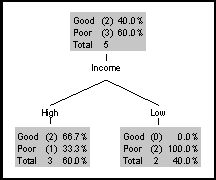
\includegraphics[width=0.3\textwidth]{img/sample_tree.jpg}
  \caption[labelInTOC]{Drzewo decyzyjne}
  \label{fig:sample_tree}
\end{center}
\end{figure}

\subsection{Om�wienie algorytm�w}
O
\subsubsection{ID3}
I
\subsubsection{C4.5}
C

\chapter{Indukcyjne bazy danych}
\section{Indukcyjne bazy danych}

% przetlumaczone z~pdf-a
Indukcyjne bazy danych �ci�le integruj� bazy danych z~koncepcj� \emph{data mining}~(\ref{lab:data_mining}).
G��wn� ich ide� stanowi to, �e zar�wno dane jak i~wzorce s� przetwarzane 
w ten sam spos�b, a~indukcyjny j�zyk zapyta� pozwala u�ytkownikowi 
na zadawanie zapyta� i~manipulacj� danymi wzorcami.

Od pocz�tku istnienia idei data miningu zdawano sobie spraw�,
�e proces ich przetwarzania powinien by� wspierany przez technologi� baz danych.
W ostatnich latach idea ta zosta�a sformalizowana jako koncepcja
\emph{indukcyjnych baz danych}.

%cytat z~artykulu
Integracja technologii baz danych z~nowoczesnymi metodami
indukcyjnego generowania wiedzy jest naturalnym kierunkiem rozwoju
system�w bazodanowych. Systemy nazywane indukcyjnymi bazami
danych potrafi� odpowiedzie� nie tylko na pytania, dla kt�rych
odpowied� znajduje si� w~bazie danych, ale r�wnie� na pytania,
kt�re wymagaj� zsyntetyzowania i~zastosowania wiedzy,
wygenerowanej przez indukcyjne wnioskowanie z~fakt�w z~bazy danych
i wcze�niejszej wiedzy~\cite{knowledge_disc}. Schemat typowej indukcyjnej
bazy danych przedstawiony jest na rysunku~\ref{fig:inddb}.

\begin{figure}[!ht]
     \centering
         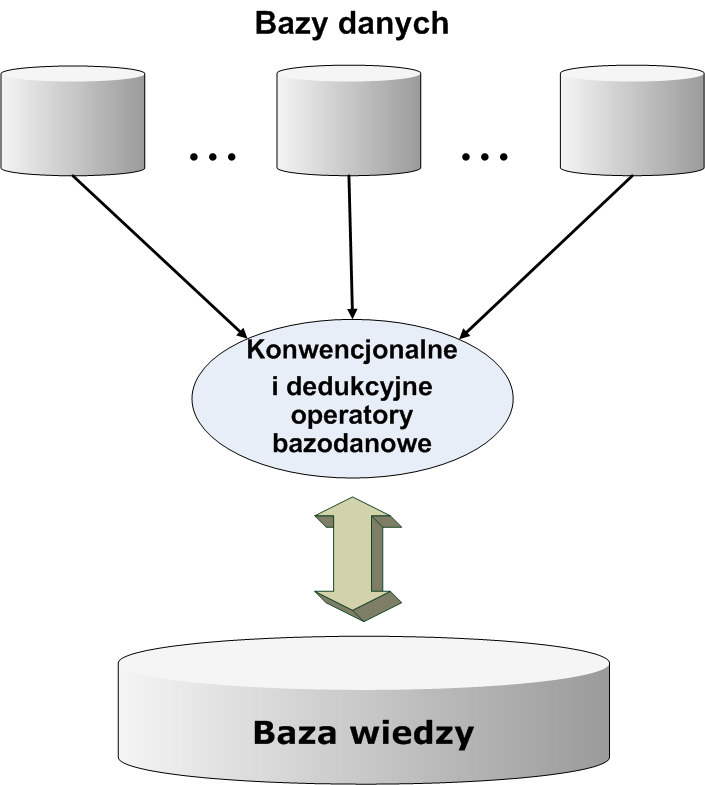
\includegraphics[width=0.90\textwidth]{img/knowledge_mining.png}
     \caption{Indukcyjna baza danych~\cite{ind_databases}}
     \label{fig:inddb}
\end{figure}

Jak zosta�o ju� wy�ej wspomniane, indukcyjne bazy danych przechowuj� nie dane
ale r�wnie� wzorce. Mo�na za�o�y�, �e zar�wno dane, jak i~wzorce stanowi� zbiory zbior�w.
To za�o�enie wynika z~analogii do tradycyjnych, relacyjnych baz danych. 
Relacyjna baza danych zawiera zbi�r relacji, kt�re to~stanowi� zbiory \emph{tupli}, 
a wi�c mo�na powiedzie�, ze stanowi zbi�r zbior�w.

W przypadku baz indukcyjnych rozr�nia si� natomiast zbi�r trenuj�cy od testuj�cego, 
zbi�r poprawnie zaklasyfikowanych przyk�ad�w od zaklasyfikowanych b��dnie itp.
 
To samo, co tyczy si� danych, odnosi si� r�wnie� do wzorc�w.
I rzeczywi�cie -- podczas procesu przetwarzania wiedzy mo�na pracowa� 
na r�nych zbiorach wzorc�w.  Zbiory te mog� odnosi� si� do odmiennych hipotez 
stworzonych na podstawie r�nych zbior�w danych,
czy r�nych ustawie� parametr�w algorytm�w je tworz�cych.

%jezyk (z pdf-a)
Jednym z~zasadniczych powod�w, kt�re przyczyni�y si� do sukcesu relacyjnych baz danych
jest opracowanie uniwersalnego j�zyka zapyta�, kt�ry podobnie jak sama algebra relacyjna
dostarcza du�ych mo�liwo�ci przy jego relatywnej prostocie.

Podobnymi cechami powinien wyr�nia� si� j�zyk zapyta� do indukcyjnych baz danych.

Rezultatem zapytania wykonanego w~takim j�zyku jest albo zbi�r wzorc�w, albo zbi�r danych.
Jest to~tak zwana \emph{w�asno�� zamkni�cia} (\emph{ ang. closure property}).
Stanowi ona analogi� do rezultat�w zapytania do relacyjnych baz danych, gdzie jest nim zawsze relacja.
Rozr�nianie mi�dzy zbiorami wzorc�w i~zbiorami danych powoduje, �e potrzebne s� dwa rodzaje zapyta�:
te kt�re generuj� zbiory wzorc�w i~zbiory danych. Zapytania do jednocze�nie obu typ�w zbior�w nazywane
s� czasami \emph{zapytaniami krzy�uj�cymi} (\emph{ang. cross-over operations}).

%dodawanie/usuwanie data setow, patternow? (patternow trudniej, nie wiem dokladnie jak, olac na razie)

%wnioskowanie
% z~pdf-a
Teoria indukcyjnych baz danych mo�e by� u�yteczna tylko w~przypadku,
gdy oferuje mo�liwo�� wnioskowania z~danych i~zgromadzonej wiedzy.
Na podstawie otrzymanej informacji trenuj�cej indukcyjna baza danych generuje now� lub 
ulepsza wcze�niej posiadan� wiedz�, w~pewien ustalony spos�b reprezentowan� 
i przeznaczon� do wykorzystania przy wykonywaniu okre�lonego zadania.
Mechanizm, zgodnie z~kt�rym dokonuje si� nabywanie lub doskonalenie wiedzy, 
jest najcz�ciej jednoznacznie wyznaczany przez metod� reprezentacji 
wiedzy oraz posta� informacji trenuj�cej \cite{ind_databases}.

\subsection{VINLEN}
\label{lab:vinlen}
Vinlen  \cite{vinlen} to system indukcyjnej bazy danych, rozwijany w
\emph{George Mason University}. Jest to~klasyczna
realizacja indukcyjnej bazy danych. Mechanizmy wnioskowania
indukcyjnego s� zintegrowane ze standardowymi relacyjnymi
operatorami bazodanowymi. Integracja ta opiera si� na nowych
rodzajach operator�w zwanych operatorami generowania wiedzy
\emph{KGO} (Knowledge Generation Operators). \emph{KGO} operuje na
\emph{segmentach wiedzy} sk�adaj�cych si� z~kombinacji jednej lub
wi�cej tabel z~relacyjnej bazy danych i~wiedzy przechowywanej
w~bazie wiedzy (por. rysunek~\ref{fig:inddb}). \emph{KGO} przyjmuje
na wyj�ciu jeden lub wi�cej segment wiedzy, na podstawie kt�rego
generuje inny segment wiedzy. Podstawowym operatorem u�ywanym w
systemie jest AQ21, program do indukcyjnego tworzenia regu� na
podstawie danych.

Indukcyjne bazy danych mog� by� wspierane przez wyspecjalizowanych
agent�w (\emph{Scauts}), kt�rych zadaniem jest synteza
i~zarz�dzanie wiedz�, kt�ra jest dostosowywana do wymaga�
okre�lonego u�ytkownika. System \emph{VINLEN} pozwala na tworzenie skrypt�w
operuj�cych na bazach danych, wiedzy i~algorytmach uczenia
maszynowego przy u�yciu j�zyka \emph{KGL-1} (\emph{Knowledge
Generation Language}).

Cech� charakterystyczn� tak rozwijanego systemu b�dzie mo�liwo��
sk�adowania wiedzy w~relacyjnej bazie danych wraz z~danymi,
zadawanie zapyta� oraz manipulowanie wiedz� z~wykorzystaniem
j�zyka \emph{KQL} lub przy u�yciu funkcjonalnego, graficznego
interfejsu u�ytkownika.


%%
\mgrclosechapter
%%
%% ==== ROZDZIA� 2 ====
%%
% \input{Mgr_roz2}
%%
%%
%% ======== DODATKI ========
%%
%%
%% ======== BIBLIOGRAFIA ========
%%
\newpage

\begin{thebibliography}{99}
\bibitem {bib2} {Kaufman, K. and Michalski, R.S., The Development
    of the Inductive Database System VINLEN: A Review of Current
    Research, International Intelligent Information Processing and
    Web Mining Conference, Zakopane, Poland, 2003}

\bibitem {bib3} {Michalski, R.S. and Kaufman, K., Data Mining and
    Knowledge Discovery: A Review of Issues and a Multistrategy
    Approach, Machine Learning and Data Mining: Methods and
    Applications, R. S. Michalski, I. Bratko and M.  Kubat (Eds.), pp.
    71-112, London: John Wiley \& Sons, 1998}

\bibitem {bib4} {Michalski, R.S., Knowledge Mining and Inductive
    Databases: An Emerging New Research Direction, School of
    Computational Sciences, George Mason University, 2004}

\bibitem {yale} {Mierswa, I., Klinkenberg, R., Fischer, S., Ritthoff, O.,
    A Flexible Platform for Knowledge Discovery Experiments:
    YALE -- Yet Another Learning Environment,
    LLWA 03 - Tagungsband der GI-Workshop-Woche Lernen - Lehren - Wissen -
    Adaptivit�t, 2003.}

\bibitem{uci} {Newman, D.J., Hettich, S., Blake, C.L., Merz, C.J.,
UCI Repository of machine learning databases, Irvine, CA, 1998.}

\bibitem {weka} {Witten, I.H., Frank, E., Data Mining: Practical Machine Learning Tools and
Techniques, Morgan Kaufmann, 2005}



\end{thebibliography}

%%
%% ======== DODATKOWE ELEMENTY PRACY (nieobowi�zkowe) ======== 
%%
%\printindex  
%%

\end{document}